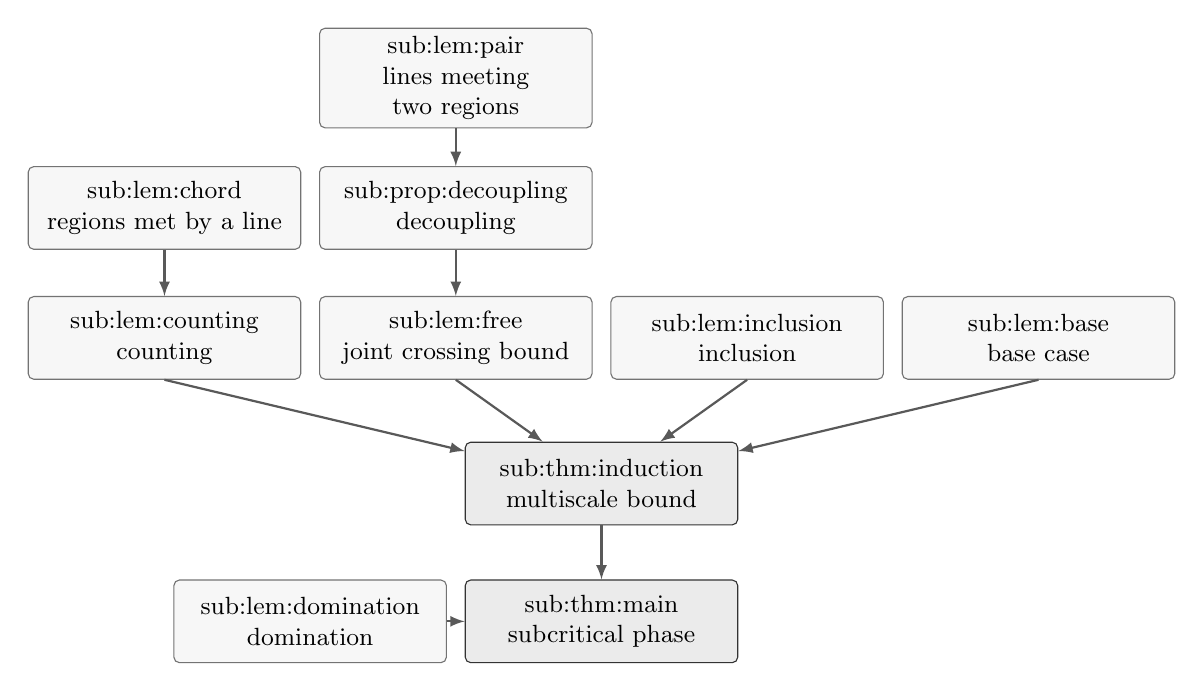
\begin{tikzpicture}[
    x=1cm,y=1cm,>=latex,
    stmt/.style={draw=black!55,fill=black!3,rounded corners=2pt,align=center,
      text width=3.25cm,minimum height=1.05cm,font=\small,inner sep=3pt},
    main/.style={stmt,draw=black!80,fill=black!8},
    dep/.style={->,thick,black!65}]
  % geometry and offsets
  \node[stmt] (pair) at (-1.85,4.6) {\cref{sub:lem:pair}\\lines meeting two regions};
  \node[stmt] (dec)  at (-1.85,2.95) {\cref{sub:prop:decoupling}\\decoupling};
  \node[stmt] (chord) at (-5.55,2.95) {\cref{sub:lem:chord}\\regions met by a line};
  % ingredients of the induction step
  \node[stmt] (count) at (-5.55,1.3) {\cref{sub:lem:counting}\\counting};
  \node[stmt] (free)  at (-1.85,1.3) {\cref{sub:lem:free}\\joint crossing bound};
  \node[stmt] (incl)  at (1.85,1.3) {\cref{sub:lem:inclusion}\\inclusion};
  \node[stmt] (base)  at (5.55,1.3) {\cref{sub:lem:base}\\base case};
  % conclusions
  \node[main] (ind)  at (0,-0.55) {\cref{sub:thm:induction}\\multiscale bound};
  \node[stmt] (dom)  at (-3.7,-2.3) {\cref{sub:lem:domination}\\domination};
  \node[main] (thm)  at (0,-2.3) {\cref{sub:thm:main}\\subcritical phase};
  \draw[dep] (pair) -- (dec);
  \draw[dep] (dec) -- (free);
  \draw[dep] (chord) -- (count);
  \draw[dep] (count.south) -- (ind);
  \draw[dep] (free.south) -- (ind);
  \draw[dep] (incl.south) -- (ind);
  \draw[dep] (base.south) -- (ind);
  \draw[dep] (ind) -- (thm);
  \draw[dep] (dom) -- (thm);
\end{tikzpicture}
